\documentclass[conference, letterpaper]{IEEEtran}
\IEEEoverridecommandlockouts
% The preceding line is only needed to identify funding in the first footnote. If that is unneeded, please comment it out.
\usepackage{cite}
\usepackage{amsmath,amssymb,amsfonts}
\usepackage{algorithmic}
\usepackage{graphicx}
\usepackage{textcomp}
\usepackage{amsmath}
\usepackage{stfloats}
\usepackage[]{algorithm2e}
\usepackage{tabularx, booktabs} 
\def\BibTeX{{\rm B\kern-.05em{\sc i\kern-.025em b}\kern-.08em
    T\kern-.1667em\lower.7ex\hbox{E}\kern-.125emX}}
\graphicspath{{./images/}}
\newcolumntype{C}{>{\centering\arraybackslash}p{1.8cm}}
\usepackage{hyperref}
\hypersetup{pdftex,colorlinks=true,allcolors=blue}
\usepackage{hypcap}

\begin{document}

\title{Estimating Baseline Travel Times for the UK Strategic Road Network
%\thanks{Thanks to EPSRC and Thales UK.}
}

\author{\IEEEauthorblockN{Alvaro Cabrejas Egea}
\IEEEauthorblockA{\textit{MathSys Centre for Doctoral Training} \\
\textit{University of Warwick}\\
Coventry, United Kingdom \\
a.cabrejas-egea@warwick.ac.uk}
\and
\IEEEauthorblockN{Peter De Ford}
\IEEEauthorblockA{\textit{Geospatial Department} \\
\textit{McKinsey \& Company} \\
	San Jose, Costa Rica \\
	pdeford@outlook.com}
\and
\IEEEauthorblockN{Colm Connaughton}
\IEEEauthorblockA{\textit{Warwick Mathematics Institute} \\
\textit{\& Centre for Complexity Science} \\
\textit{University of Warwick}\\
Coventry, United Kingdom \\
c.p.connaughton@warwick.ac.uk}
}

\maketitle

\begin{abstract}
We present a new method for long-term estimation of the expected travel time for links on highways and their variation with time.  
The approach is based on a time series analysis of travel time data from the UK's National Traffic Information Service (NTIS).  
Time series of travel times are characterised by a noisy background variation exhibiting the expected daily and weekly patterns punctuated by large spikes associated with congestion events. 
Some spikes are caused by peak hour congestion and some are caused by unforeseen events like accidents. 
Our algorithm uses thresholding to split the data into background and spike signals, each of which is analysed separately. 
The the background signal is extracted using spectral filtering. 
The periodic part of the spike signal is extracted using locally weighted regression (LWR). 
The final estimated travel time is obtained by recombining these two. 
We assess our method by cross-validating in several UK motorways. 
We use 8 weeks of training data and calculate the error of the resulting travel time estimates for a week of test data, repeating this process 4 times. 
We find that the error is significantly reduced compared to estimates obtained by simple segmentation of the data and compared to the estimates published by the NTIS system.
\end{abstract}

\begin{IEEEkeywords}
Travel Time, Traffic Congestion, Prediction
\end{IEEEkeywords}

\section{Introduction}
The UK collects and processes data from its Strategic Road Network (SRN) in real time and makes it available through the National Traffic Information Service (NTIS) \cite{NTIS}. 
NTIS collects speed, flow and travel time data using sensors on the road and in vehicles. 
The basic building blocks of the SRN are called links -  segments of motorway between 500 and 20000 metres in length.  
NTIS data is used to assign a travel time profile to each link. 
Profiles should represent the typical time to traverse a link at a given time of day on a given day of the week and are the topic of study of this paper.
 
Profiles clearly vary with day of the week and time of the day but should be relatively stable from one week to the next.
This stability over time means calculating profiles is different from the problem of short-term forecasting.
While there is no a-priori mathematical definition of a typical travel time,  we take it to mean the value that minimises the mean absolute percentage error (MAPE) with respect to subsequently measured travel times.
NTIS publishes profile values alongside measured travel times although the methodology used to calculate them is not in the public domain. 
In this paper, we present a novel method for generating profiles for a complete week. 
Our approach is based on statistical analysis of previous data and does not require any a-priori segmentation of days into classes. 
Rather patterns of intra- and inter-day variability are learned directly from the data.

The available literature on travel times is extensive but most recent research focuses on short-term forecasting and not on the long term \cite{long-term} \cite{long-term-2}. 
From a methodological point of view machine learning and statistical methods take most of the attention \cite{should}, different approaches can be found: using historical data \cite{simple} \cite{dynamic-historic}, neural networks \cite{NN}.
Others take closer approaches to this paper differentiating between peak and non-peak \cite{peak-historic}, using spectral analysis \cite{spectral1} \cite{spectral2} or Locally Weighted Regressions \cite{williams} \cite{sun} \cite{zhong} \cite{chowdhury} \cite{acqua} \cite{vana}.
Comparisons between some of these studies and others can be found in \cite{nikovski}, \cite{lint}, \cite{mori} and \cite{ser}. 
Most of these methods have been specifically tuned for the conditions on which they have been developed and transferability to other sites is often not evaluated.
To assess the transferability of our method, it is tested on three different motorways.
The method here presented, uses a combination of spectral analysis, tree decisions and local regression.
\section{Examples of travel times} 
The most direct variable for measuring the state of traffic over a length of road is the vehicles' travel times. 
The instantaneous travel time for a given segment of road is the average time that the vehicles currently in it are taking since they enter the segment until they exit it.\\

\begin{figure}[htbp]
	\centerline{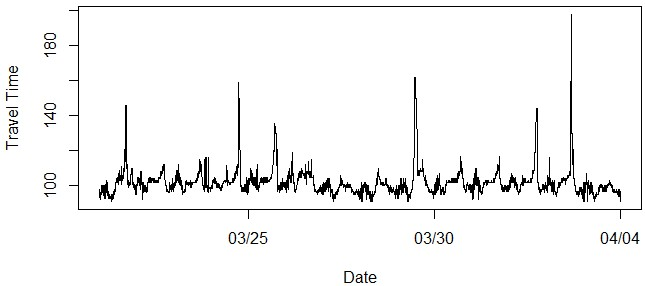
\includegraphics[width=\linewidth]{./images/Traveltime_example2.jpg}}
	\caption{Travel times on link 117007401 in the M6 over three weeks.}
	\label{fig:travel_time_example}
\end{figure}

As it can be seen in Figure \ref{fig:travel_time_example} the travel time remains within a vaguely predictable pattern most of the days, with bounded minima during nights corresponding with the free flow time and with some outliers below this value corresponding to speeding drivers. 
Travel time will meaningfully rise as people leave to work and add load to the motorways. 
This collective behaviour will create the morning traffic jams, which in our data, are partially replicated during the evening rush hour, normally finding a plateau in between. 
After this, the travel times slowly decay towards the night period of free-flow regime.
In Figure \ref{fig:travel_time_example}, it can also be seen that there are a series of excursions out of this oscillating yet bounded typical behaviour. 
In these, the travel time can increase several times fold the usual values.
These extreme oscillations are much less predictable both in intensity and inter-oscillation period than the recurrent congestion described previously.

\section{Basic methods for profile estimation}
\subsection{Use of Exponentially Weighted Moving Average (EWMA)} \label{ewma}
The most basic approach to profile estimation is to apply an EWMA on the same minute of every day, with the implicit assumption that similar behaviour is expected at the same time of the day. 
In this approach, the estimated profile $\hat{x}(i,d+1)$ on the $i-th$ minute of a given day $d$, for a memory parameter $\alpha \in [0,1]$ and with measured travel time $x_i^d$, will be:
\begin{equation}
\hat{x}^{d+1}_i = \alpha * x^{d}_{i} + (1-\alpha)*\hat{x}^{d}_{i}
\end{equation}
The main problem with EWMA is the manner in which the memory decays. 
Recent measurements are weighted more heavily than events in the past. Thus if an extreme fluctuation occurs,  the following profile estimates will be biased, partially replicating this event and over-estimating the travel times until enough new measurements arrive to dissipate this effect.
\subsection{Segmentation}\label{segmentation}
In addition, to acknowledge the specific differences between some special dates in the year, and the difference between days of the week, this family of methods requires the use of heavy date based segmentation. 
The EWMA will be applied across dates which fall in the same category (i.e. Mondays, weekends, Christmas Day, ...).
If this is combined with the shortcomings presented in Section \ref{ewma}, some long reaching effects are generated, which can propagate for weeks into the future predictions, but do not have any reflection on the observed travel times. A possible instance of this effect can be seen in Figure \ref{fig:EWMA_spike}.
Furthermore, in order to generate a valid segmentation, an experienced team is necessary, since the needs of the process can geographically vary, given that the EWMA approach tends to better approximate endemic congestion. 
This dependence can lead to the creation of legacy systems which may not be well understood after a few years, decreasing their usability over time unless extra effort is put into transmitting this knowledge and continually train new staff.
\begin{figure}
	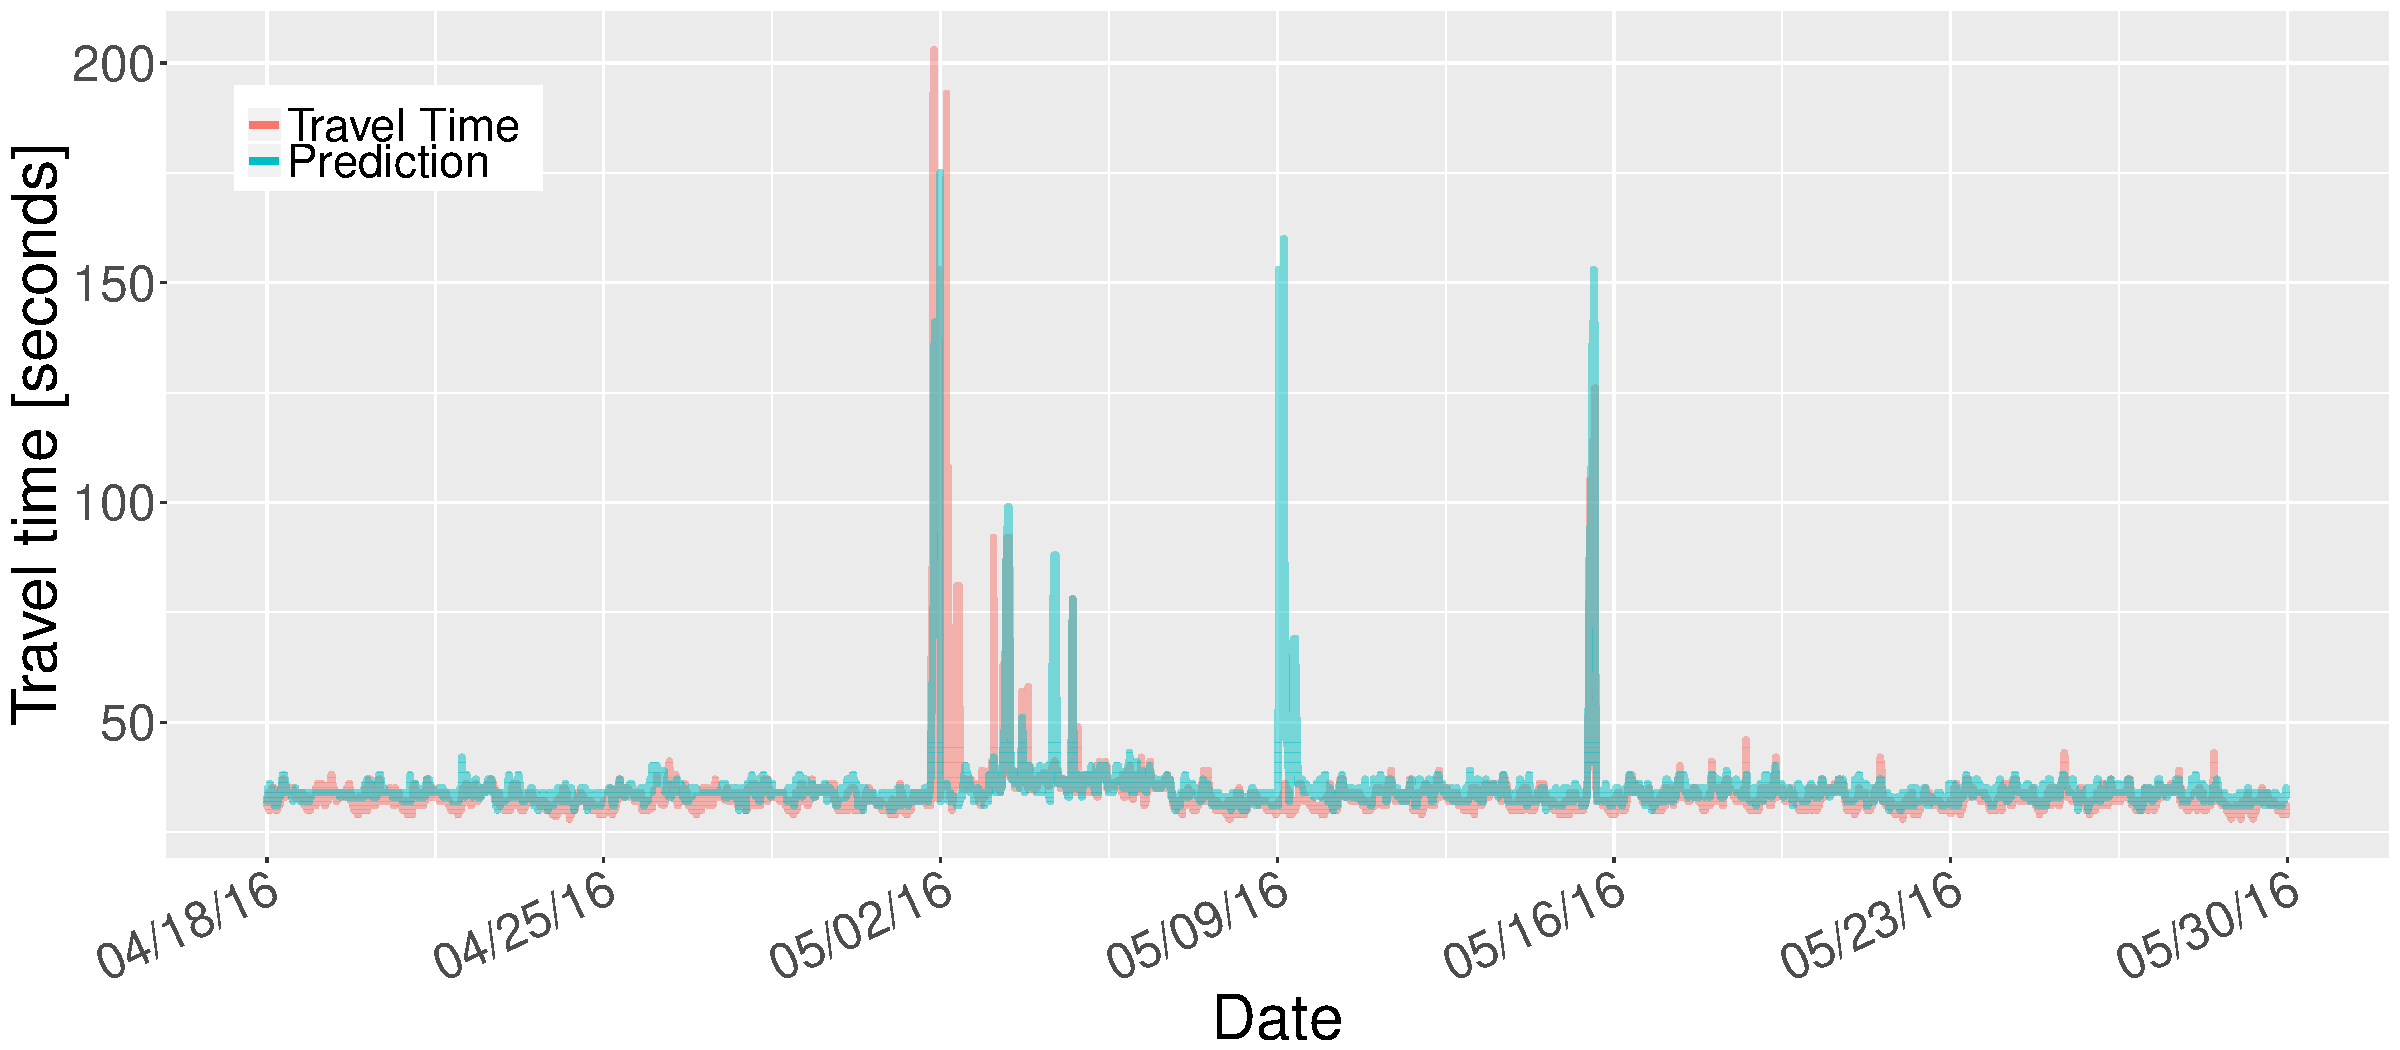
\includegraphics[width=\linewidth]{EWMA.pdf}
	\caption{A single large random spike in travel time can lead to over-estimation of subsequent profile estimates.}
	\label{fig:EWMA_spike}
\end{figure}
\section{Data}
\subsection{Data Gathering and Selection}
Data was gathered from 3 different Motorways in England.
The M6 and M11 were selected due to their high usage and combination of recurrent and outstanding congestion. 
The M25 was selected on the base that it is the most used Motorway in England on a daily basis, suffering from chronic congestion.
\begin{itemize}
	\item The dataset for M6 comprises 90 days (12 complete weeks) of data (07/03/2016-05/06/2016) across 14 links.
	\item The dataset for d M11 comprises 90 days (12 complete weeks) of data (07/03/2016-05/06/2016) across 25 links.
	\item The dataset for M25 comprises 75 days (10 complete weeks) of data (07/04/2017-20/06/2017) across 61 links.
	\item Links were discarded if they had more than 10\% of missing data or if they contained any entry or exit ramps.
	\item Whenever missing data was detected for 10 or less minutes, it was linearly interpolated.
	\item Whenever missing data was detected for over 10 minutes, it was left as missing values.
\end{itemize}
In the case of the M6 and the M11 the first 8 weeks are used to predict one complete week ahead.
One week later, the process is repeated, deleting the oldest week of training data and incorporating measurements of the week predicted in the previous step. This is performed 4 times.
In the case of the M25, 6 weeks of data were used for training and the process as described above is performed 3 times.
\subsection{Data Contents}
For each link on a specific date, the required input data consists of one entry per minute, containing:
\begin{itemize}
	\item Measured travel time
	\item Profile (expected) travel time 	
\end{itemize}
\section{Travel Time Prediction Algorithm} \label{algorithm}

\begin{figure}[htbp]
	\centerline{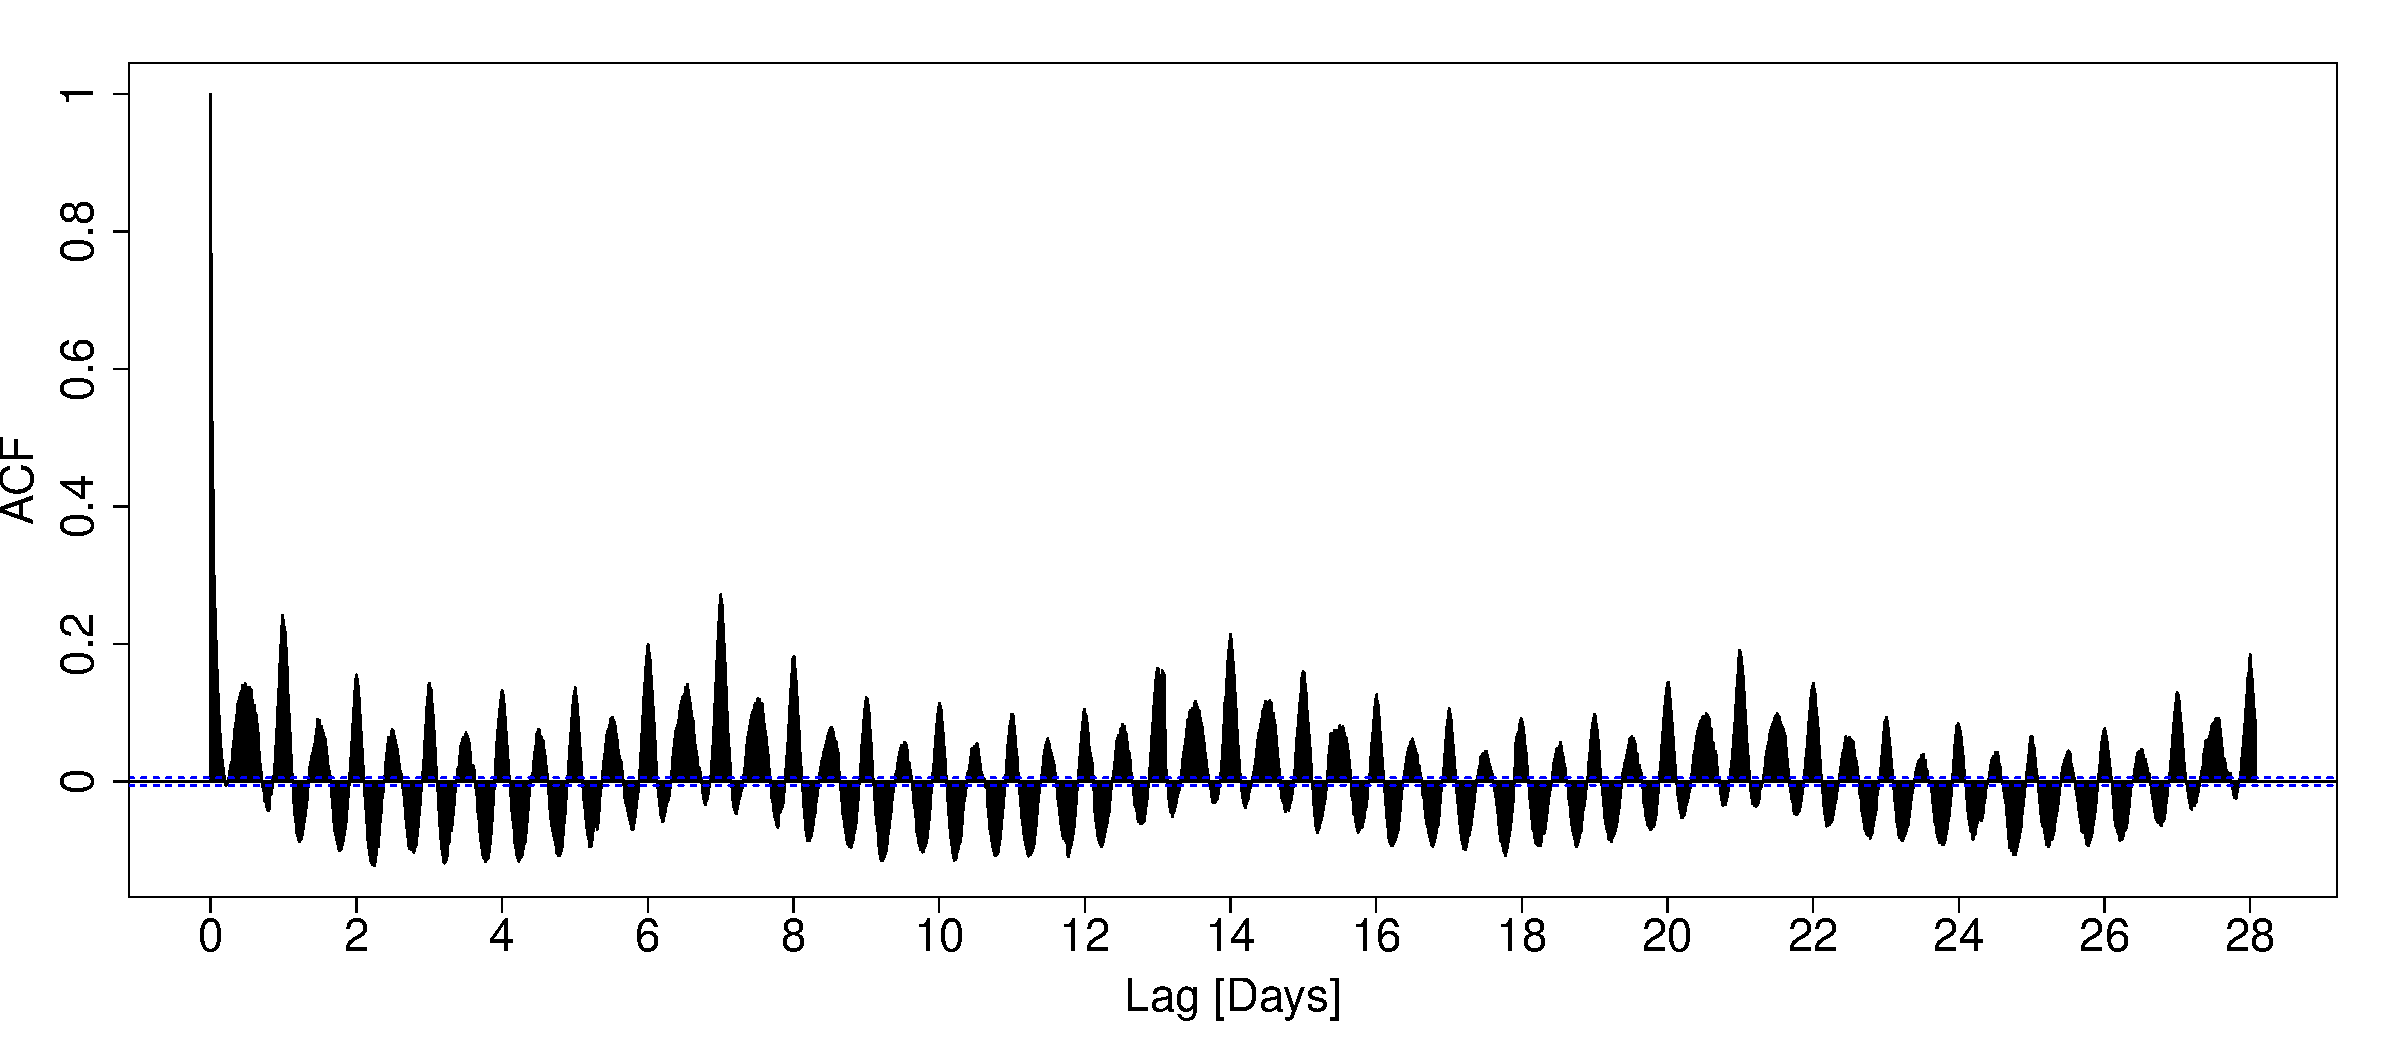
\includegraphics[width=\linewidth]{./images/finalplots/ACF_M6_Link3.pdf}}
	\caption{Autocorrelation function of a link in the M6 over a period of 4 weeks, showing seasonal patterns on the daily and weekly periods.}
	\label{fig:acf}
\end{figure}

Given the cyclic nature of traffic, the aim was a prediction algorithm that could account for the periodic variations and endemic congestion while being resilient to fluctuations and rare events. This algorithm also should:
\begin{itemize}
	\item Be robust, mitigating the propagation of isolated events into future forecasts, unlike methods using EWMA.
	\item Not require the use of time segmentation and be valid for regular and "special" dates.
	\item Be location agnostic, the internal parameters should be set algorithmically based on the data.
	\item Have Gaussian, mean 0, uncorrelated residuals.
	\item Near flat Trend term, given the different time scales between seasonal cycles and changes in the general motorway flow.
\end{itemize}

\subsection{Naive Segmentation}
To obtain an accurate comparison of the performance of the algorithm developed in the following subsections, an example of basic segmentation was coded. 
This involved a weighted combination of the training data points using uniform weights. 
In this way, for the $i-th$ minute of a week and using a training set composed of the previous of $n$ weeks, the Naive Segmentation (NS) profile is:
\begin{equation}
\hat{x}(i,n) = \sum_{\textrm{week}=1}^{n} \frac{x^i_n}{n} 
\end{equation}

\subsection{Decomposition in Background and Spikes}
During exploratory data analysis we found that, from the point of view of travel times, traffic operates in two differentiated regimes that we denominated Background and Spikes. 
\begin{itemize}
	\item Background: 
	\begin{itemize}
		\item Stable around a mean value.
		\item Oscillates with small amplitude and high frequency.
		\item Suitable for spectral filtering.
	\end{itemize}
	\item Spikes: 
	\begin{itemize}
		\item Zero most of the time. Quickly go to extreme values.
		\item Oscillates with great amplitude and low inter-oscillation frequency, creating far reaching effects.
		\item Suitable for seasonal decomposition.
	\end{itemize}
\end{itemize}

\begin{figure}[htbp]
	\centering
	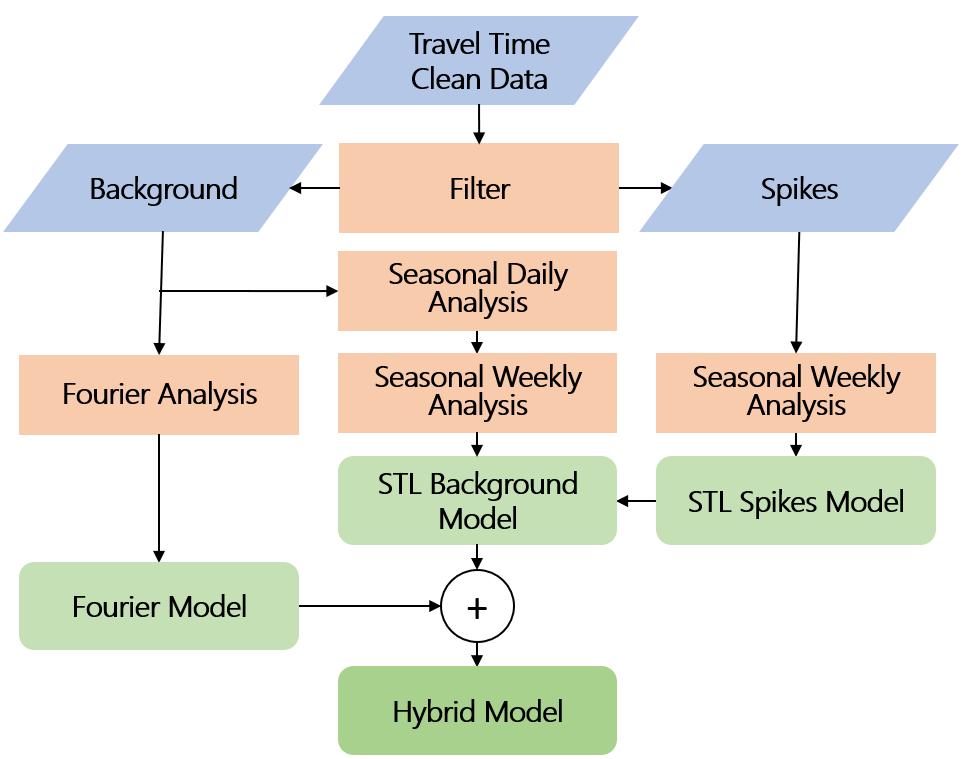
\includegraphics[width=\linewidth]{new_flow2.png}
	\caption{Schematic of data streams in the algorithm.}
	\label{fig:flowchart}
\end{figure}

This decomposition, assuming Gaussian noise $\xi$, signal of the form:
\begin{equation}
\textrm{Travel Time}_t  = \textrm{Background}_t + \textrm{Spikes}_t + \xi
\end{equation}
The objective was to separate them in such a way that times of smooth operation are captured as part of the Background and used for spectral analysis, attempting to mitigate the prediction error induced by the high frequency oscillations and obtaining a basic view of what can be daily observed.
Meanwhile, the spikes, including the recurring and non-recurring congestion, were treated separately searching for seasonality in larger time scales than those in which the background oscillates, as suggested by Fig. \ref{fig:acf}. 
Ideally, after this step, the remainder should only contain isolated large rare events deviating from the profile and white noise.\\

To prevent the differing lengths of the links from affecting this decomposition, for this step, all travel times were normalized according to their corresponding link's free flow time, defined as the time to transverse the length of the link at the maximum legal speed allowed by the motorway. 
However, this step only mitigates the non-regularity of the time series, since there are drivers who do not follow these limits.
A threshold was heuristically set, as seen in Table \ref{table:threshold}  to separate the two components in the different regimes from the normalised travel times on a per-motorway basis, although better results can be obtained by setting each link individually. 
Intuitively, this threshold scales with the amount of recurring congestion in a link. Whenever a data point was above the threshold, it was flagged as belonging to a spike.
\begin{table}[htbp]
	\caption{Travel Time Normalisation Thresholds}
	\begin{center}
		\begin{tabular}{|c|c|}
			\hline
			\textbf{Motorway}&{\textbf{Threshold}} \\
			\hline
			M6& 1.1\\
			\hline
			M11& 1.2\\
			\hline
			M25& 1.4\\
			\hline
		\end{tabular}
		\label{table:threshold}
	\end{center}
\end{table}


\begin{figure}[htbp]
	\centering
	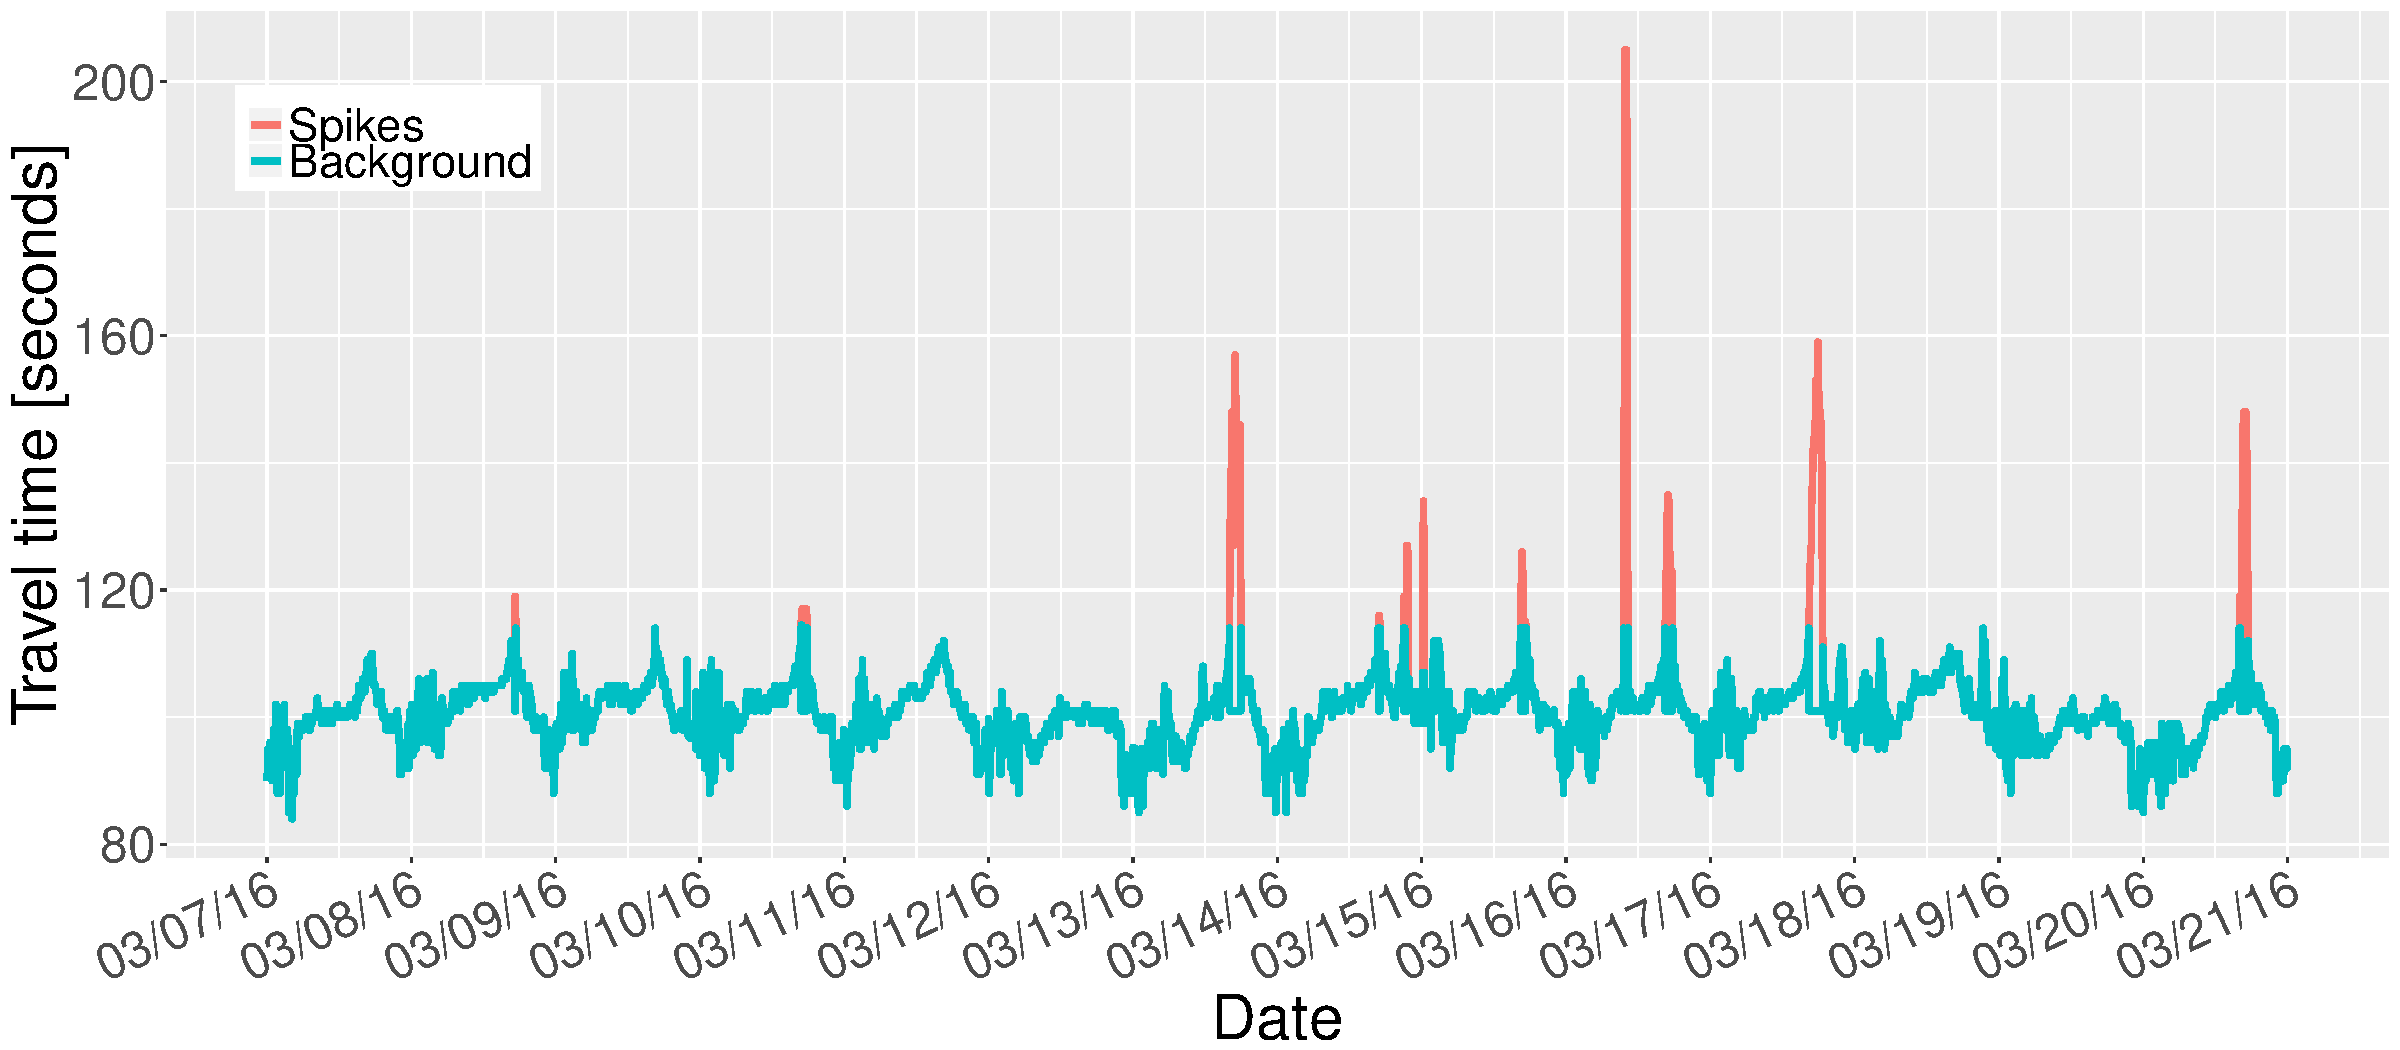
\includegraphics[width=\linewidth]{BS.pdf}
	\caption{ Decomposition time series in background and spikes }
	\label{fig:Background}
\end{figure}

For this purpose, an indicator function was defined, taking for every minute the value:
\begin{equation}
    \delta_t^{spike}=
    \begin{cases}
      1, & \text{if } x_t > \text{Threshold}\\
      0, & \text{otherwise}
    \end{cases}
    \label{delta}
  \end{equation}

\subsection{Spectral Component}
The main difficulty when dealing with the Background signal is the low amplitude, high frequency fluctuations that can be found almost ubiquitously. 
Signal smoothing can be performed by completely removing a range of frequencies while the information bearing bands are retained. For this task, the Fast Fourier Transform (FFT) \cite{FFT} was used as follows:
\begin{enumerate}

	\item Calculate Background Power Spectrum using FFT
	\item Remove frequencies corresponding to periods under 4 hours and over 1 week
	\item Repeat for all $n$ weeks in training set
    \item Apply EWMA to the modified weekly Power Spectra
	\item Compute the Inverse Transform

\end{enumerate}
\subsection{Seasonality Component}
Seasonal-Trend Decomposition based on LOESS (STL) \cite{STL} was chosen for the seasonality analysis since it can handle any type of seasonality, allowing the user to control how it changes over time as well as the smoothness of the trend-cycle while being robust to outliers \cite{forecasting}.\\

Below, the sequence of steps taken to extract the Seasonality Components that can be observed in Fig. \ref{fig:acf} is described in line with Fig. \ref{fig:flowchart}. 
Note that this should be applied to the $n$ training weeks as a single time series.
\begin{enumerate}
	\item Decomposition of Background for daily seasonality
	\item Extract and sum the series corresponding Trend and Remainder from Step 1
	\item Decomposition of output from 2 for weekly seasonality
	\item Add daily and weekly Seasonal components from Step 1 and Step 3 to obtain global seasonality
	\item Average seasonality across training weeks
	\item Linearise Trend term from output of Step 3
	\item Add linearised trend to seasonality obtained in Step 6
	\item STL Decomposition of Spikes for weekly seasonality
	\item Extract Spike's Seasonality corresponding to the number of weeks for forecasting
	\item Add Spike's Seasonal component to the output of 8
\end{enumerate}
To ensure a successful decomposition, after Step 3  Background's Remainder should be zero mean, Gaussian distributed. Background's Trend should have a near zero slope. This should also hold after Step 8.
\subsection{Seasonal-Spectral Hybrid Profile}
In order to create the final Seasonal-Spectral Hybrid profile (Hybrid), one of the two forecasts generated in the previous points is taken, depending on what is the identified regime: 

\begin{equation}
\textrm{Hybrid} = \textrm{Seasonal} * \delta_{\textrm{spike}} + \textrm{Spectral} * (1 - \delta_{\textrm{spike}})
\end{equation}

\section{Accuracy Results}
\begin{table*}[bp]
	\caption{MARE Distribution Per Motorway}
	\centering
	\begin{center}
		\begin{tabular}{|C|C|C|C|C|C|C|C|C|}
			\hline
			\textbf{\% rel. error}&{\textless -25\%}&{-25\%\textbf{ to }-15\%}&{-15\%\textbf{ to }-5\%}&{-5\%\textbf{ to }5\%}&{5\%\textbf{ to }15\%}&{15 \%\textbf{ to }25\%}&{\textgreater 25\%}\\
			\hline
			M6& 1.58& 0.60& 3.77& 88.01& 5.97& 0.06& 0.01\\
			\hline
			M11& 0.80& 0.35& 4.07& 86.15& 7.97& 0.49& 0.15\\
			\hline
			M25& 3.85& 2.73& 10.42& 75.12& 7.29& 0.33& 0.28\\
			\hline
		\end{tabular}
		\label{mapeglobal}
	\end{center}
\end{table*}
  
In this section the accuracy of the algorithm described above is compared against the Published Profiles and the NS Model. 
For each temporal point $i$, the Mean Average Relative Error (MARE) is defined below:
\begin{equation}
\textrm{MARE} =\frac{ \left( \sum_{i=1}^{n} \frac{\|x_i - \hat{x_i}\|}{x_i}\right)}{n}
\end{equation}
For complete Motorways, the Root Mean Squared Error (RMSE) has been calculated for each temporal point $i$ as:
\begin{equation}
\textrm{RMSE} = \sqrt{\frac{\sum_{i=1}^{n} (x_i - \hat{x_i})^2}{n}}
\end{equation}

In both cases the error for a Link is defined as the average MARE or RMSE across all prediction points.
The error for a Motorway is defined as the average of the error across all its links.
\subsection{Accuracy by Quantile}
\begin{figure}[htbp]
	\centerline{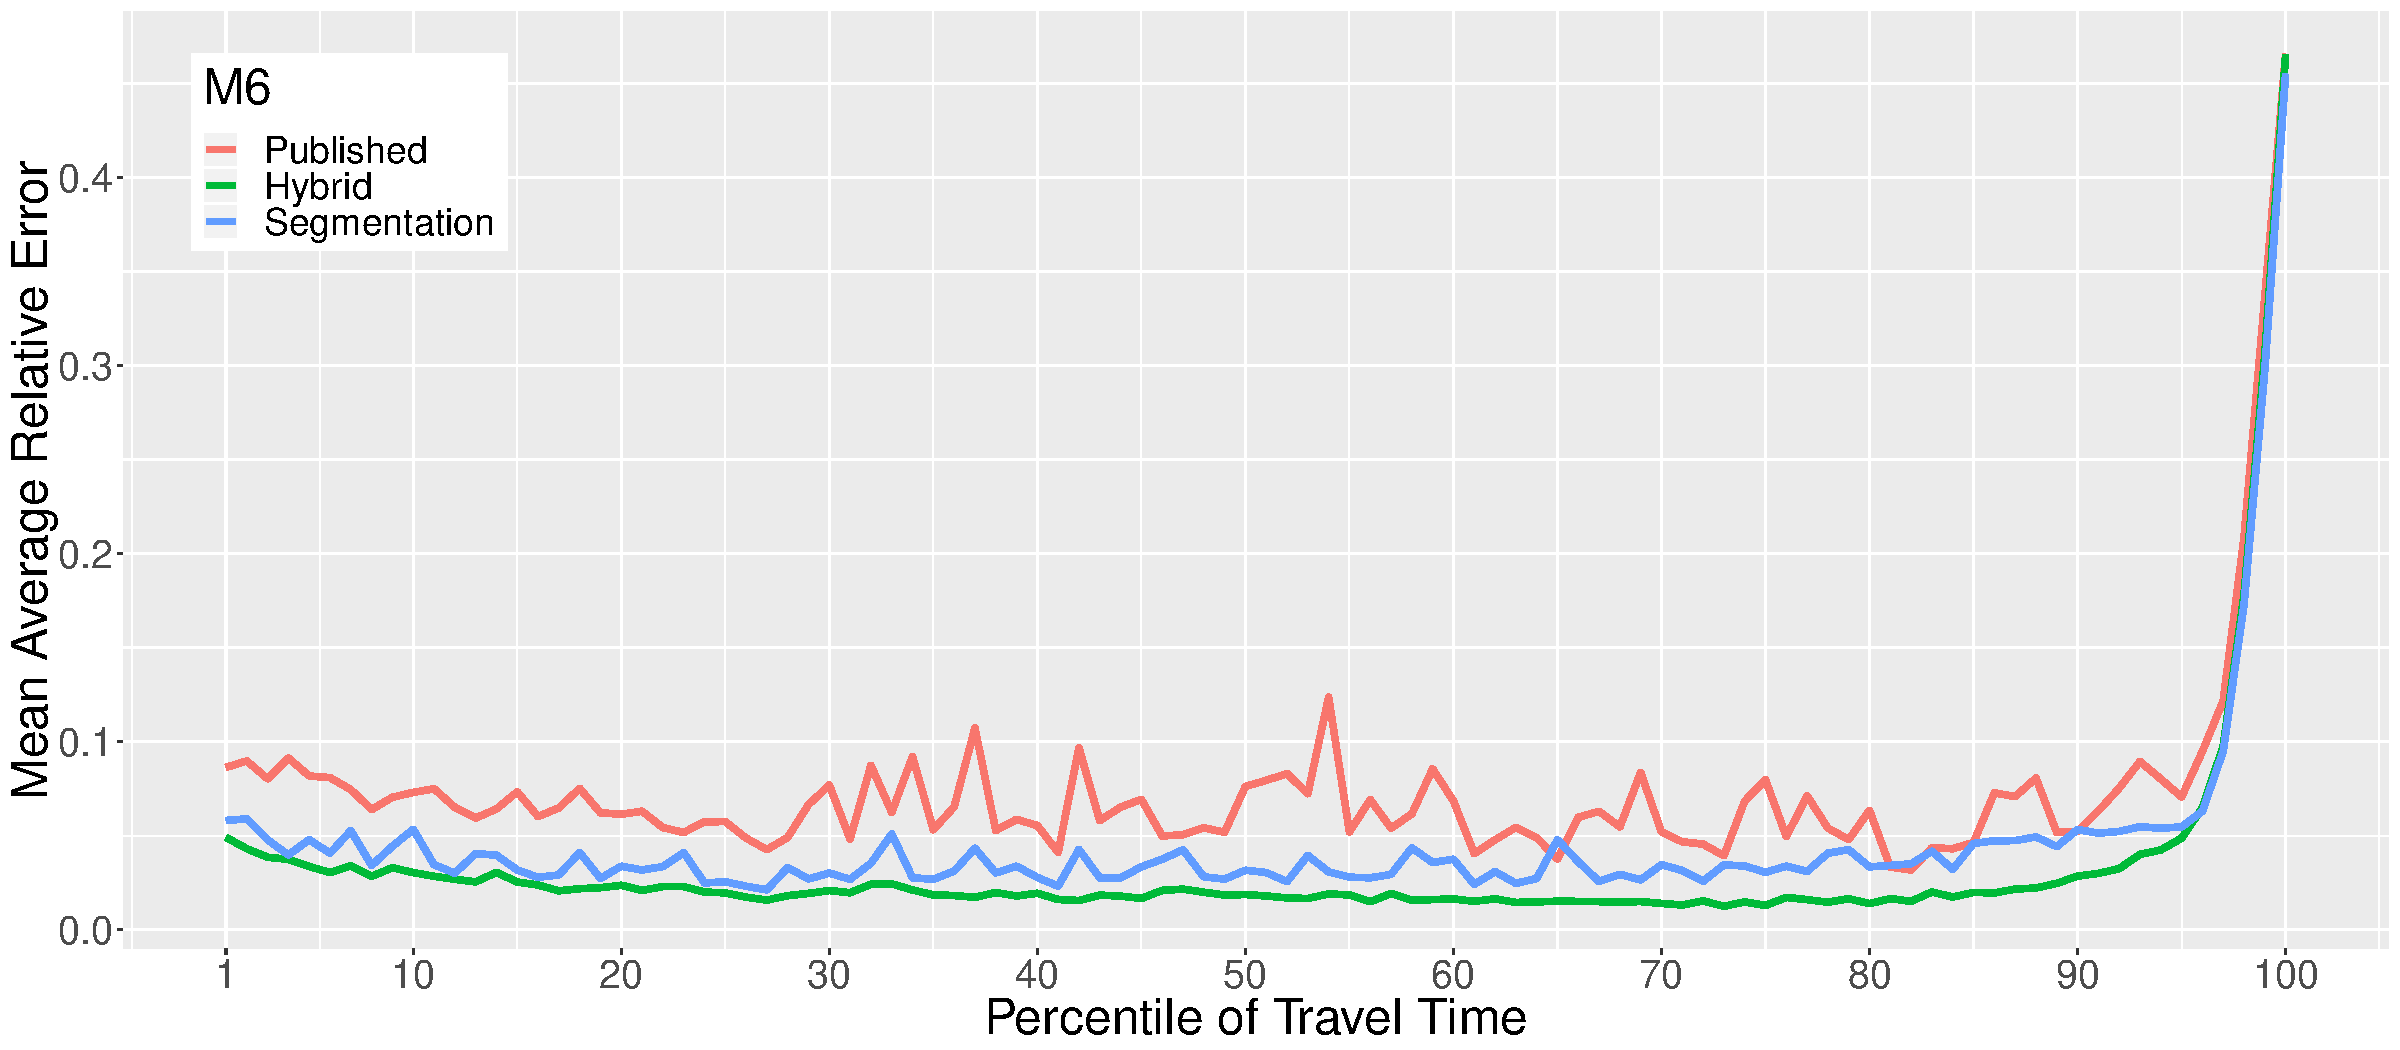
\includegraphics[width=\linewidth]{/finalplots/m6_q2.pdf}}
	\caption{Average accuracy results in M6 across percentiles of travel time.}
	\label{fig:m6q}
\end{figure}

\begin{figure}[htbp]
	\centering
	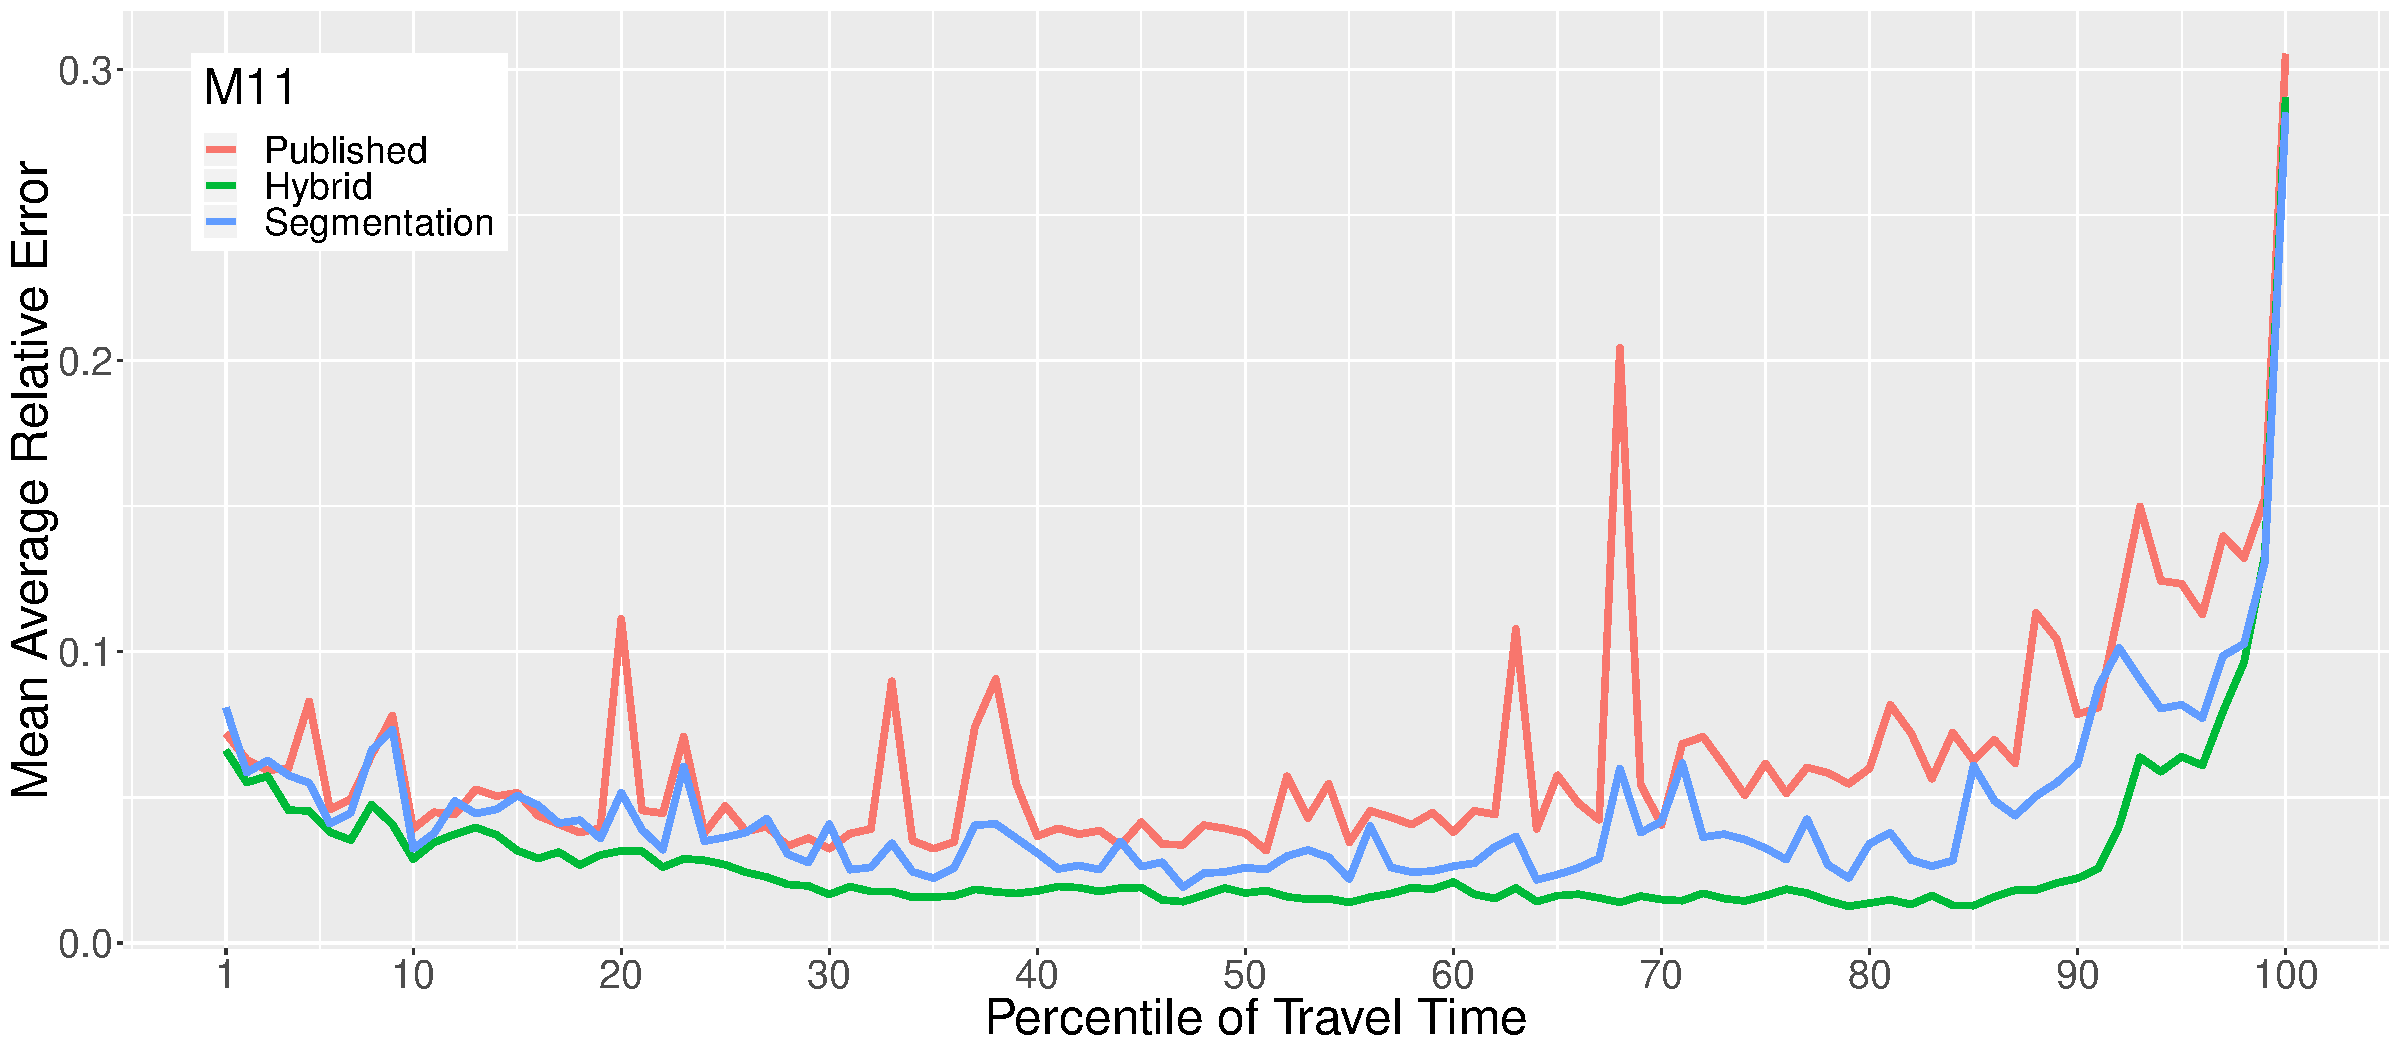
\includegraphics[width=\linewidth]{/finalplots/m11_q2.pdf}
	\caption{Link average accuracy results in M11 across percentiles of travel time.}
	\label{fig:m11q}
\end{figure}

\begin{figure}[htbp]
	\centering
	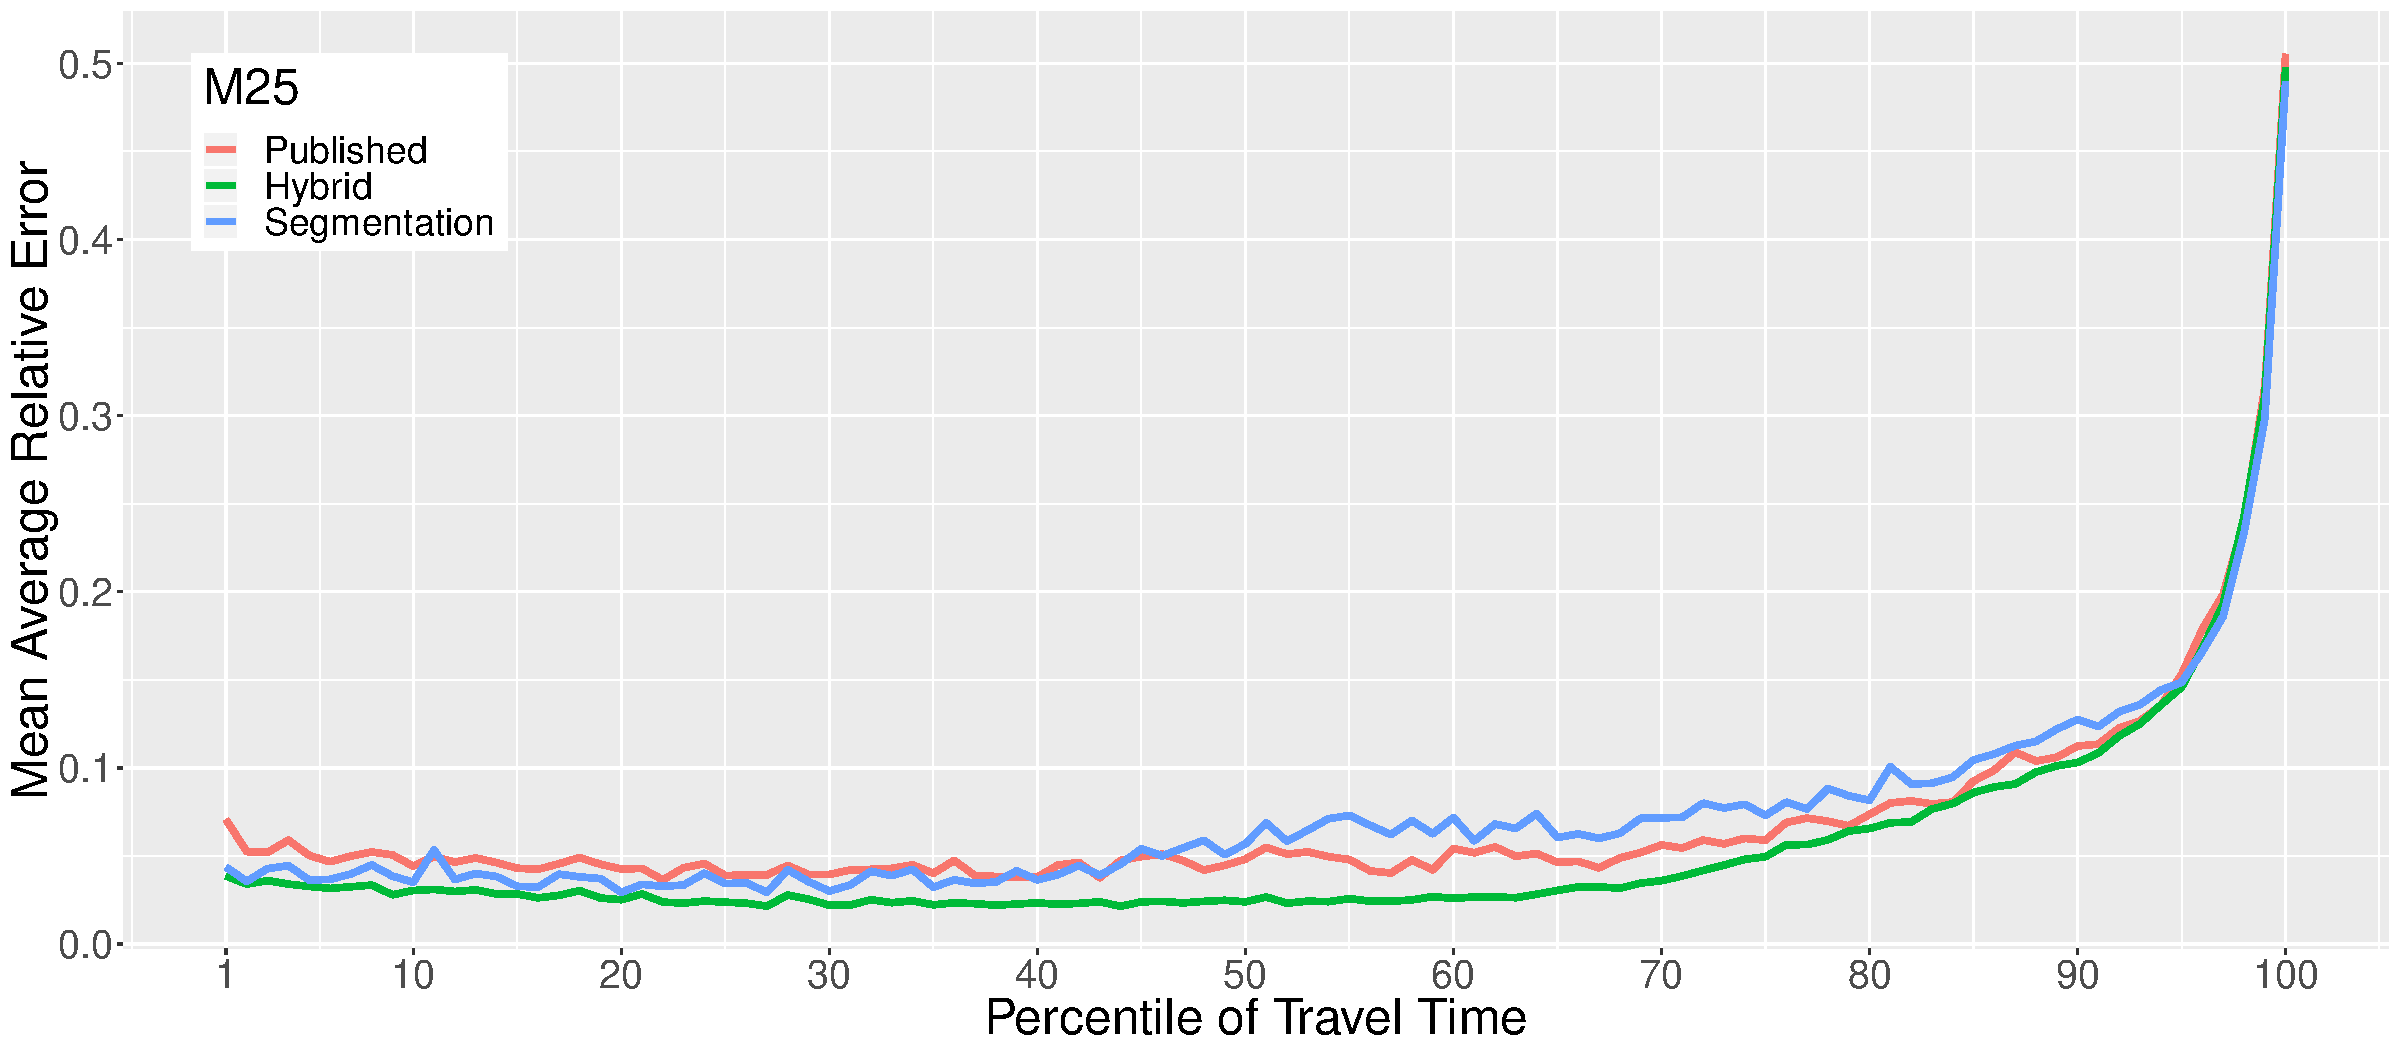
\includegraphics[width=\linewidth]{/finalplots/m25_q2.pdf}
	\caption{Link average accuracy results in M25 across percentiles of travel time.}
	\label{fig:m25q}
\end{figure}
Here, the accuracy of the algorithm is compared against the Published Profiles and the NS Profile across all percentiles of travel time.
As it can be seen in Figs. \ref{fig:m6q}, \ref{fig:m11q} and \ref{fig:m25q}, the Hybrid Profile has a higher accuracy than the Published Profiles and the NS Model for all percentiles of travel time except for the most extreme values where they all perform poorly.\\
The most meaningful difference occurs between percentiles $[50-95]$, where the Published Profile starts to suffer from higher inaccuracy.

\subsection{Daytime Error}
\begin{figure}[htbp]
	\centering
		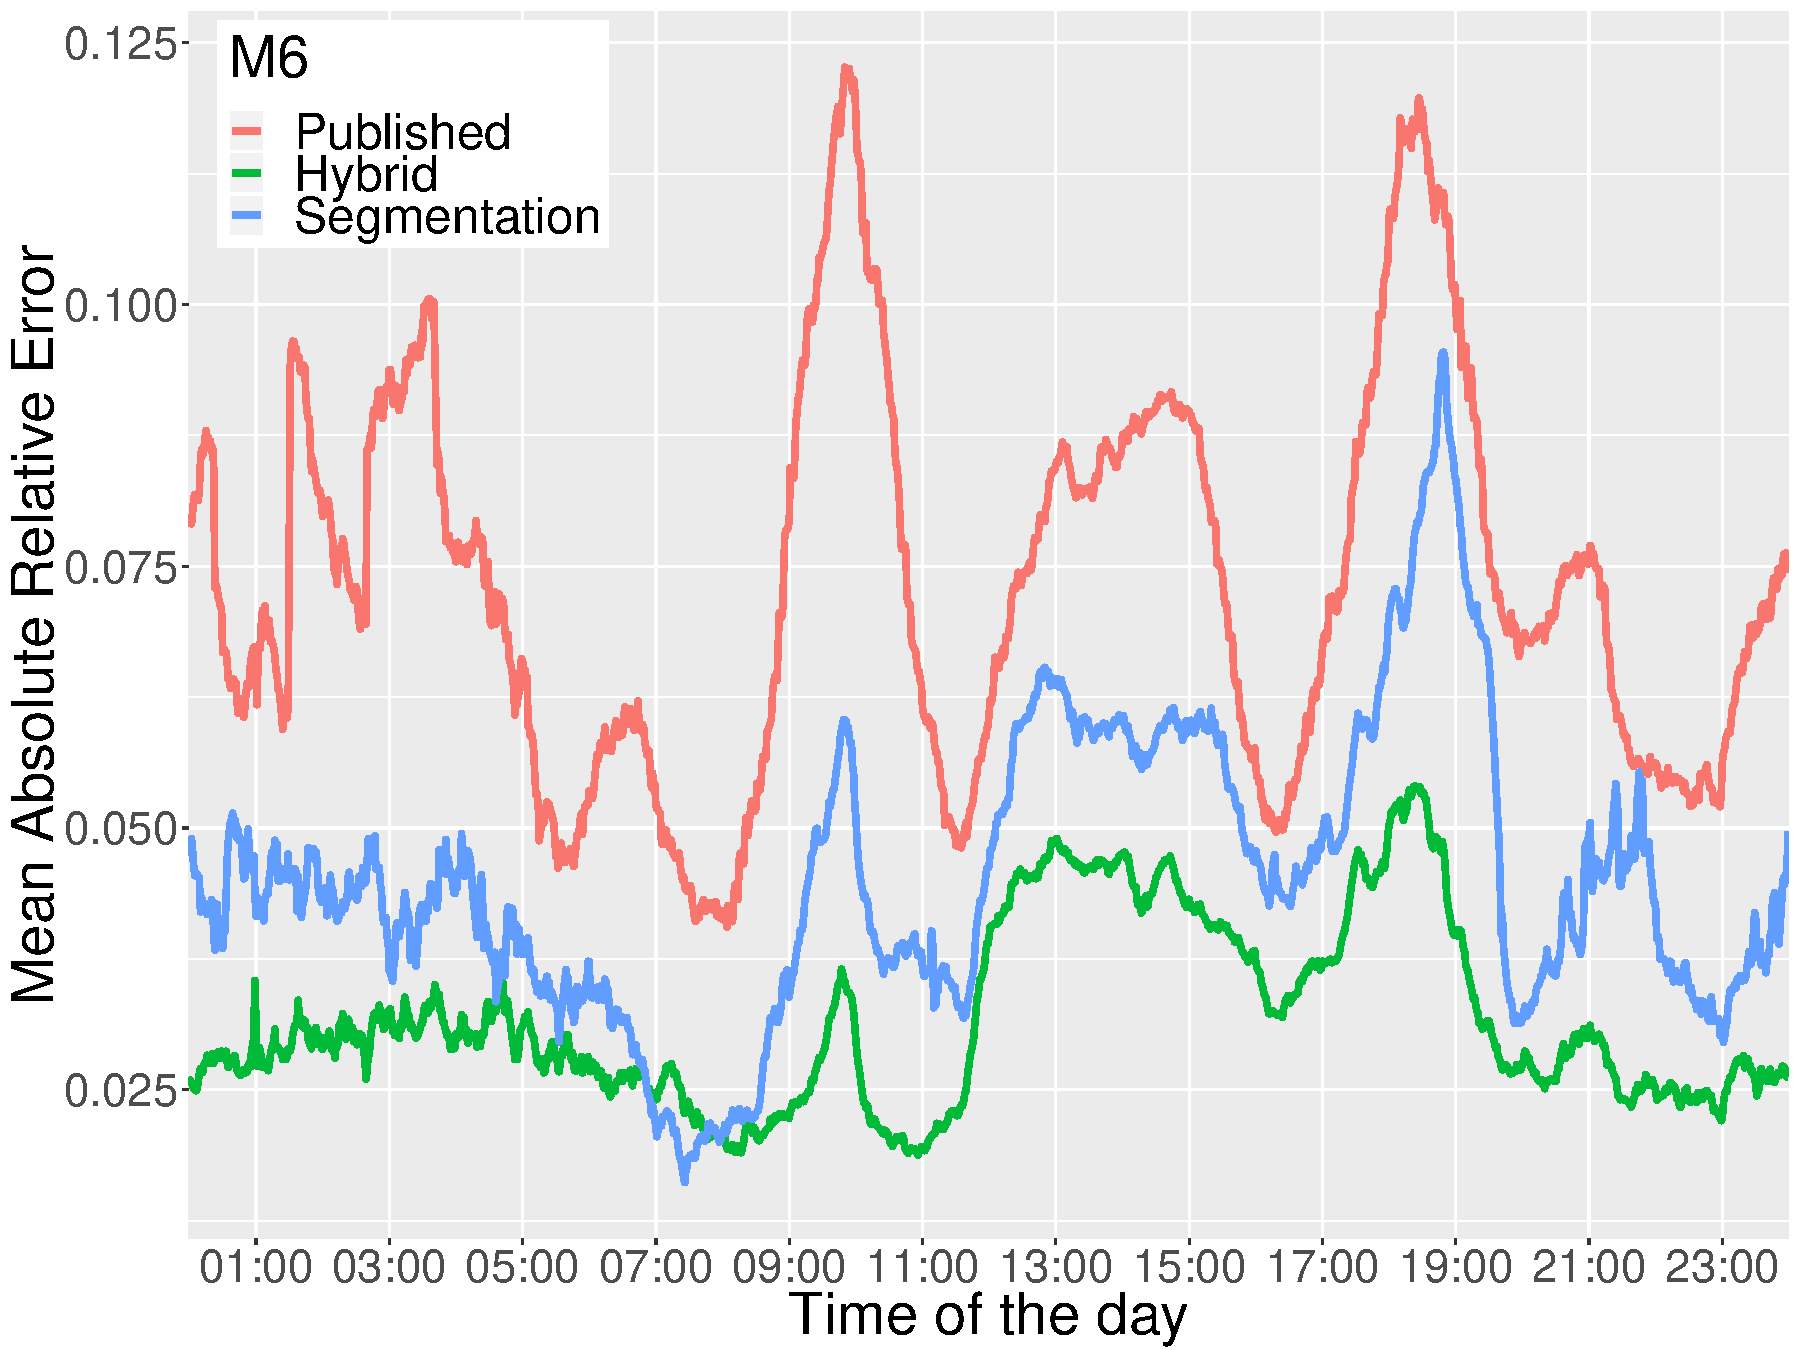
\includegraphics[width=\linewidth]{/finalplots/m6_dt2.pdf}
	\caption{Link average accuracy results in M6 across times of the day.}
	\label{fig:m6daytime}
\end{figure}

\begin{figure}[htbp]
	\centering
	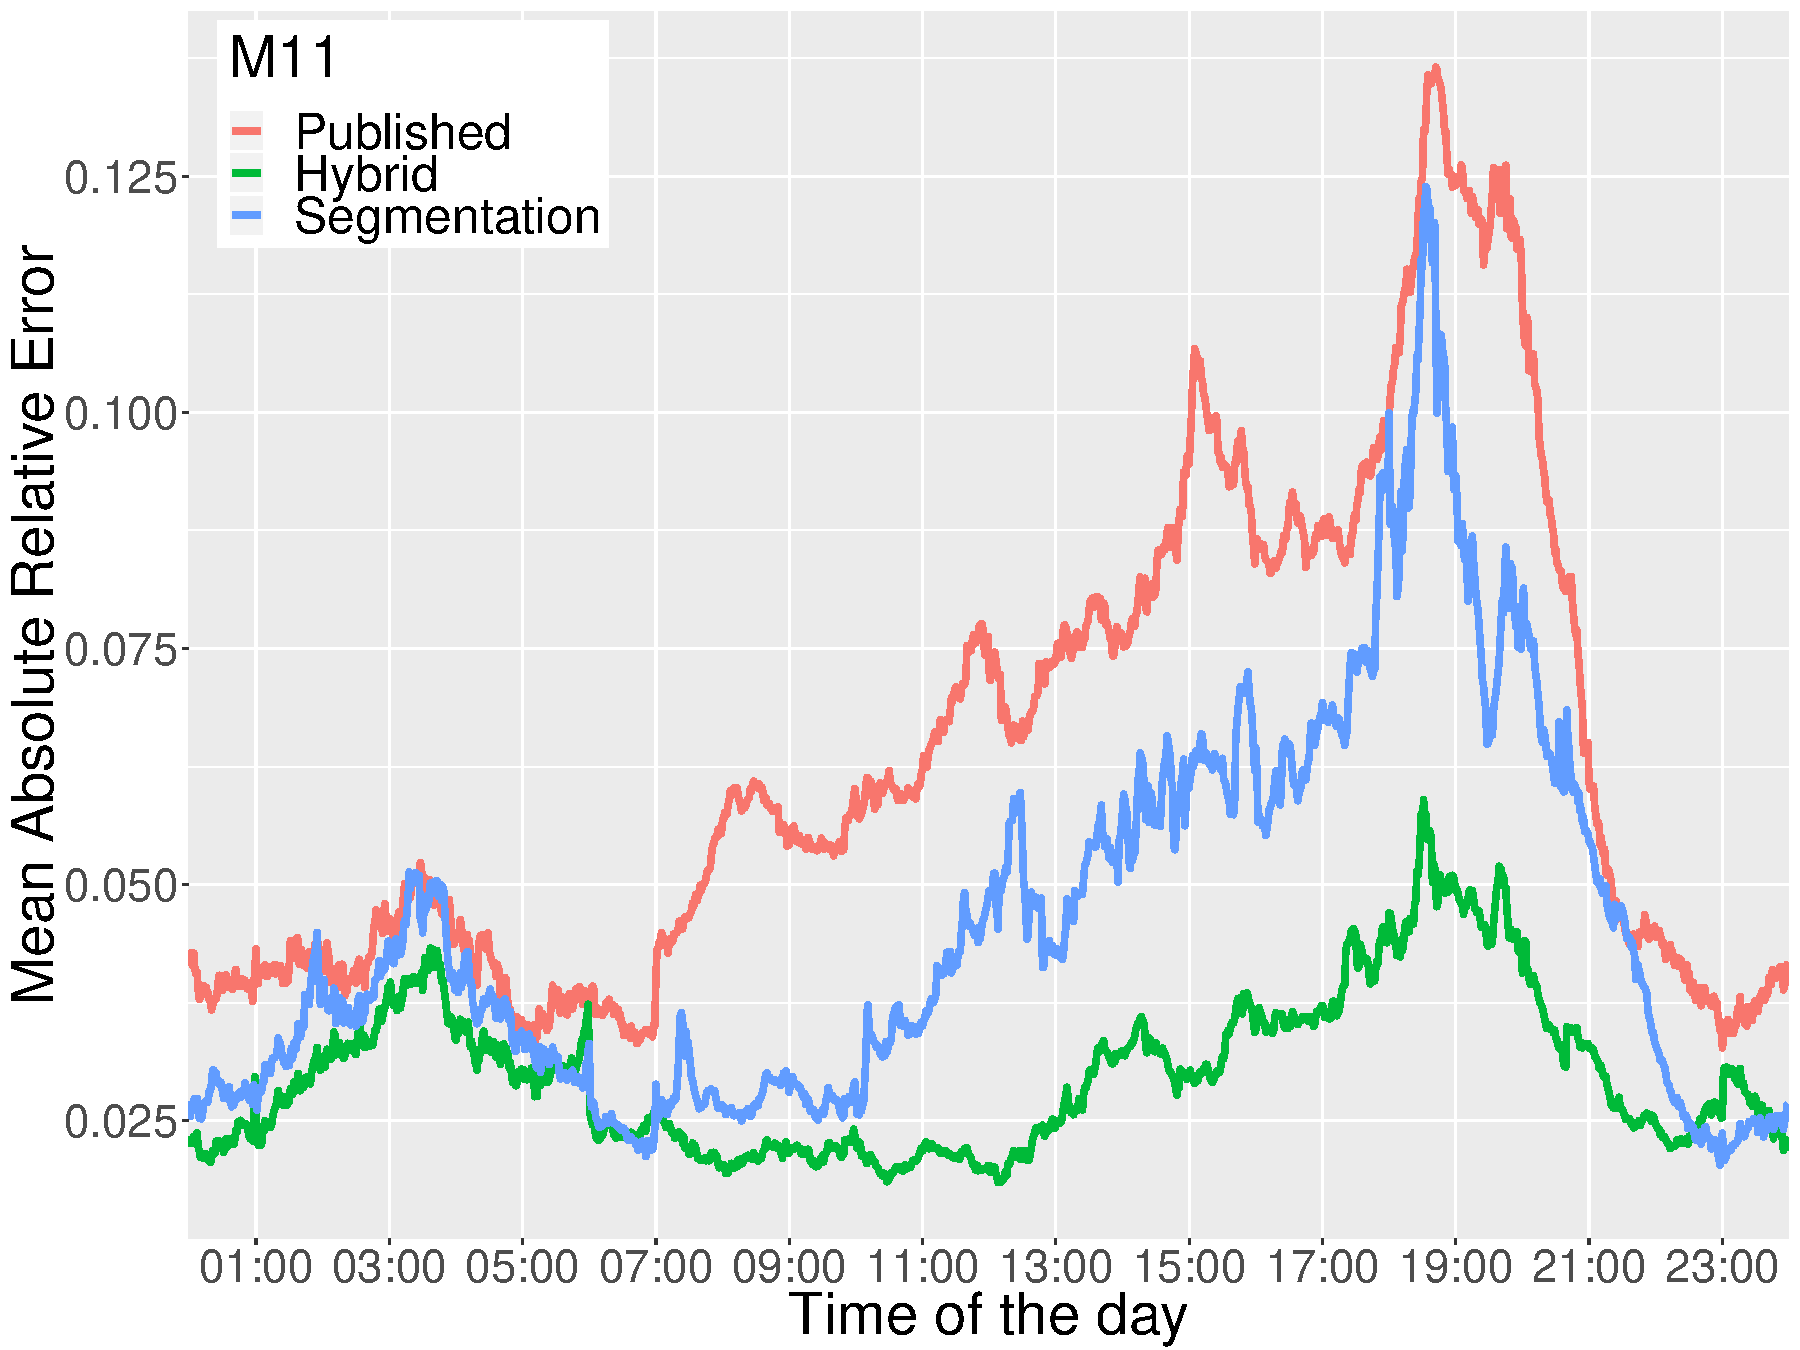
\includegraphics[width=0.95\linewidth]{/finalplots/m11_dt2.pdf}
	\caption{Link average accuracy results in M6 across times of the day.}
	\label{fig:m11daytime}
\end{figure}

\begin{figure}[htbp]
	\centering
	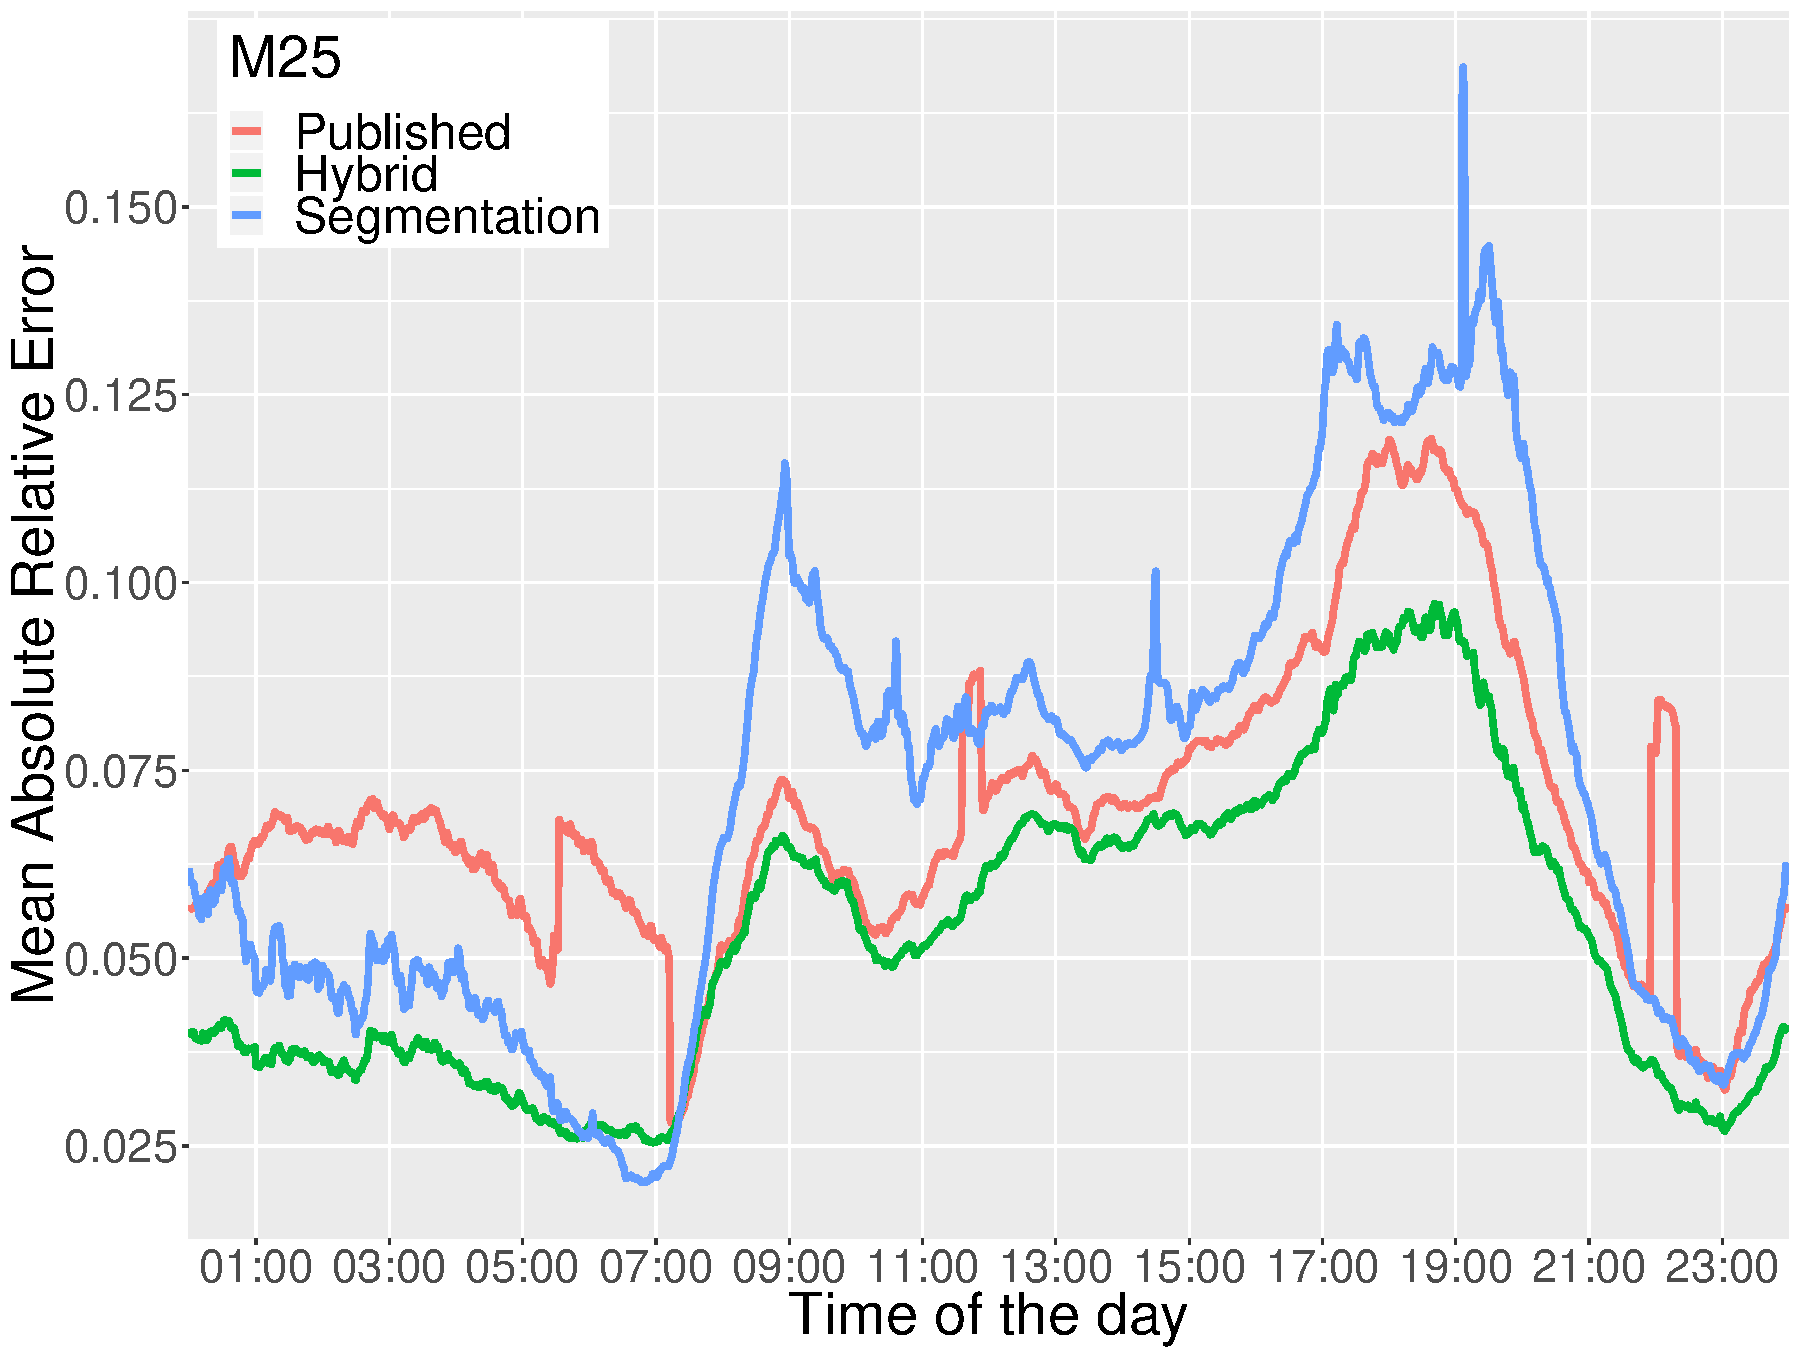
\includegraphics[width=\linewidth]{/finalplots/m25_dt2.pdf}
	\caption{Link average accuracy results in M25 across times of the day.}
	\label{fig:m25daytime}
\end{figure}

Here, the accuracy of the algorithm is compared against the Published Profiles and the NS Profile across the times of the day.
As it can be seen in Figures \ref{fig:m6daytime}, \ref{fig:m11daytime} and \ref{fig:m25daytime}, the Hybrid Profile has a higher accuracy than the Published Profiles and the NS Model for all times of the day, all locations and training lengths. 
The most relevant improvement occurs during the morning and evening peak hours, where the algorithm presented in this paper does not accuse meaningful performance worsening relative to the morning plateau when compared with the other two profiles.\\
In the case of the M6 and M11, where the training set is richer, the error at peak times is reduced by at least 50\% in all cases, reaching as much as 68.7\% in the case of the M6 morning rush.
In the case of the M25, which is congested on a regular basis, the errors in the Published Profile during peak times are slightly lower than on the other cases, indicating that, given the use of EWMA, this recurrent congestion is better captured by it. 
Even in this case, the proposed algorithm performs significantly better than any of the other two, except for a brief window between 6-7AM when it is outperformed by the NS Model.

\begin{table}[htbp]
	\caption{MARE per Link on M6}
	\begin{center}
		\begin{tabular}{|c|c|}
			\hline
			\textbf{Link}&{\textbf{MARE}} \\
			\hline
			117007401& 0.0211\\
			\hline
			117007501& 0.0421\\
			\hline
			117007601& 0.0246\\
			\hline
			117007801& 0.0480\\
			\hline
			117007901& 0.0308\\
			\hline
			117008401& 0.0331\\
			\hline
			117009102& 0.0269\\
			\hline
			117011901& 0.0235\\
			\hline
			117012001& 0.0446\\
			\hline
			117012101& 0.0262\\
			\hline
			117012201& 0.0431\\
			\hline
			117012301& 0.0275\\
			\hline
			117016001& 0.0360\\
			\hline
			123025901& 0.0189\\
			\hline
		\end{tabular}
		\label{tab1}
	\end{center}
	\label{table:m6mape}
\end{table}

\begin{table}[htbp]
	\caption{Global MARE \& RMSE per Motorway}
	\begin{center}
		\begin{tabular}{|c|c|c|}
			\hline
			\textbf{Motorway}&{\textbf{MARE}}&{\textbf{RMSE [s]}} \\
			\hline
			M6& 0.0318& 0.0368\\
			\hline
			M11& 0.0300& 0.0355\\
			\hline
			M25& 0.0552& 0.0667\\
			\hline
		\end{tabular}
		\label{mapeglobal}
	\end{center}
\end{table}

\section{Future Work}
The algorithm presented above meets the requirements described in Section \ref{algorithm} except for an heuristically set threshold. 
One potential way of reaching compliance with these requirements is to perform the decomposition by applying a Wavelet Transform and separating background from spikes based on statistical analysis of the transformed time series in terms of how their Wavelet coefficients oscillate over time within a scale level. 
In the future a sensitivity analysis should be conducted to explore the limits of the algorithm in terms of minimum training data set, as well as maximum performance with increased training.
\section*{Acknowledgments}
This work was part funded by the EPSRC under grant no. EP/L015374. 
We are also grateful to the London Mathematical Laboratory for additional financial support. 
We thank Ayman Boustati, Laura Guzman and Guillem Mosquera for assistance with exploratory data analysis. 
We also thank Steve Hilditch and Thales Ground Transportation Systems, UK for help understanding the NTIS system.  
A. C. E. thanks Stefan Grosskinsky for the initial guidance, discussions and support.


\begin{thebibliography}{00}
\bibitem{NTIS} The Highways Agency, "National Transport Information System Publish Services", Technical Report, 2011. 
\bibitem{STL} R. B. Cleveland, W. S. Cleveland, J. E. McRae and I. Terpenning, "STL: A Seasonal-Trend Decomposition Procedure Based on Loess", Journal of Official Statistics, vol. 6, 1990, pp. 3-73.
\bibitem{forecasting} R. J. Hyndman and G. Athanasopoulos, "Forecasting: Principles and Practice", Otexts, 2013.
\bibitem{FFT} J. W. Cooley and J. W. Tukey, "An algorithm for the machine calculation of complex Fourier series", Mathematics of computation, 1965, vol. 19, no 90, p. 297-301.
\bibitem{long-term} J. Moreira, A. Jorge, J. Sousa, C. Soares 2012. Comparing state-of-the-art regression methods for long term travel time prediction. Intelligent Data Analysis. 16. 10.3233/IDA-2012-0532. 
\bibitem{long-term-2} G. Klunder, P. Baas, F. op de Beek. 2018. A long-term travel time prediction algorithm using historical data. 14th World Congress on Intelligent Transport Systems, ITS 2007; Beijing; China; October 2007 through 13 October 2007, 1191-1198
\bibitem{should} Kirby, H. R., Watson, S. M., Dougherty, M. S. 1997. Should we use neural networks or statistical models for short-term motorway traffic forecasting?. International Journal of Forecasting, 13(1), 43-50.
\bibitem{simple} Rice, J., Van Zwet, E. (2004). A simple and effective method for predicting travel times on freeways. IEEE Transactions on Intelligent Transportation Systems, 5(3), 200-207.
\bibitem{dynamic-historic} Chien, S. I. J. et al. 2003. Dynamic travel time prediction with real-time and historic data. Journal of transportation engineering, 129(6), 608-616.
\bibitem{NN} Lee, Y. 2009. Freeway travel time forecast using artifical neural networks with cluster method. In Information Fusion, 2009. FUSION'09. 12th International Conference on (pp. 1331-1338). IEEE.
\bibitem{peak-historic} Zhang, Y. et al. 2011. Analysis of peak and non‐peak traffic forecasts using combined models. Journal of Advanced Transportation, 45(1).
\bibitem{spectral1} Nicholson, H., Swann, C. D. 1974. The prediction of traffic flow volumes based on spectral analysis. Transportation Research, 8(6), 533-538.
\bibitem{spectral2} Park, D. et al. 1999. Spectral basis neural networks for real-time travel time forecasting. Journal of Transportation Engineering, 125(6).
\bibitem{williams} Williams, B., Durvasula, P., Brown, D. (1998). Urban freeway traffic flow prediction: application of seasonal autoregressive integrated moving average and exponential smoothing models. Transportation Research Record: Journal of the Transportation Research Board, (1644), 132-141.
\bibitem{sun} Sun, H., Liu, H. X., Xiao, H., He, R. R., Ran, B. (2003, January). Short term traffic forecasting using the local linear regression model. In 82nd Annual Meeting of the Transportation Research Board, Washington, DC.
\bibitem{zhong} Zhong, M., Sharma, S., Lingras, P. (2005). Refining genetically designed models for improved traffic prediction on rural roads. Transportation planning and technology, 28(3), 213-236.
\bibitem{chowdhury} Chowdhury, N. K., Nath, R. P. D., Lee, H., Chang, J. (2009, September). Development of an effective travel time prediction method using modified moving average approach. In International Conference on Knowledge-Based and Intelligent Information and Engineering Systems (pp. 130-138). Springer, Berlin, Heidelberg.
\bibitem{acqua} Dell'Acqua, P., Bellotti, F., Berta, R., De Gloria, A. (2015). Time-aware multivariate nearest neighbor regression methods for traffic flow prediction. IEEE Transactions on Intelligent Transportation Systems, 16(6), 3393-3402.
\bibitem{vana} Kumar, S. V., Vanajakshi, L. (2015). Short-term traffic flow prediction using seasonal ARIMA model with limited input data. European Transport Research Review, 7(3), 21.
\bibitem{nikovski} Nikovski D, Nishiuma N, Goto Y, Kumazawa H. Univariate short-term prediction of road travel times. Intelligent Transportation Systems, 2005. Proceedings. 2005 IEEE 2005 Sep 13 (pp. 1074-1079). IEEE.
\bibitem{lint} van Hinsbergen, C.P.IJ., van Lint, J.W.C.,  Sanders, F. M. (2007). Short Term Traffic Prediction Models. ITS World Congress, Beijing, China.
\bibitem{mori} Mori U, Mendiburu A, Álvarez M, Lozano JA. A review of travel time estimation and forecasting for Advanced Traveller Information Systems. Transportmetrica A: Transport Science. 2015 Feb 7;11(2):119-57.
\bibitem{ser} Lana I, Del Ser J, Velez M, Vlahogianni EI. Road Traffic Forecasting: Recent Advances and New Challenges. IEEE Intelligent Transportation Systems Magazine. 2018;10(2):93-109.
\end{thebibliography}

\end{document}
